\documentclass[aspectratio=169]{beamer}
\usepackage[T1]{fontenc}
\usepackage{lmodern}
\usepackage{graphicx}
\graphicspath{{docs/}}
\usepackage{xcolor}
\usepackage{amsmath}
\usepackage{tikz}
\usetikzlibrary{arrows.meta,positioning,fit}

% Nord-inspired slide colors, matching docs/design.tex
\definecolor{NordBody}{HTML}{4C566A}
\definecolor{NordBlue}{HTML}{5E81AC}
\definecolor{NordRed}{HTML}{BF616A}
\definecolor{NordGreen}{HTML}{A3BE8C}
\definecolor{NordOrange}{HTML}{D08770}
\definecolor{NordPurple}{HTML}{B48EAD}
\definecolor{NordPanel}{HTML}{ECEFF4}

\setbeamertemplate{footline}{
  \hspace{1em}%
  \usebeamercolor[fg]{page number in head/foot}%
  \usebeamerfont{page number in head/foot}%
  \insertframenumber\,/\,\inserttotalframenumber%
  \vskip2pt%
}
\beamertemplatenavigationsymbolsempty{}

\setbeamercolor{normal text}{fg=NordBody}
\setbeamercolor{title}{fg=NordBlue}
\setbeamercolor{frametitle}{fg=NordBlue}
\setbeamercolor{structure}{fg=NordBlue}
\setbeamercolor{itemize/enumerate body}{fg=NordBody}
\setbeamercolor{itemize item}{fg=NordBlue}

\hypersetup{colorlinks=true,allcolors=NordBlue}

\newcommand{\um}{\ensuremath{\mu\mathrm{m}}}
\newcommand{\placeholder}[2]{%
  \begin{tikzpicture}
    \node[minimum width=#1,minimum height=#2,draw=NordBlue!60,rounded corners=2pt,fill=NordPanel,align=center,text=NordBody]
      {Placeholder\\[-1pt]\scriptsize image not yet available};
  \end{tikzpicture}%
}
\newcommand{\maybeimage}[2][]{%
  \IfFileExists{#2}{\includegraphics[#1]{#2}}{\placeholder{0.95\linewidth}{0.30\textheight}}%
}

\title{FRIDA ADC Measurement Status}
\author{Kennedy Caisley}
\date{\today}

\begin{document}

% ============================================================
\begin{frame}
  \frametitle{FRIDA Test Chip Overview}
  \begin{columns}[T,onlytextwidth]
    \begin{column}{0.50\textwidth}
      \centering
      \maybeimage[width=\linewidth,height=0.72\textheight,keepaspectratio]{images/frida_65A.png}
      \vspace{2pt}

      {\small Layout view}
    \end{column}
    \begin{column}{0.50\textwidth}
      \centering
      \maybeimage[width=\linewidth,height=0.72\textheight,keepaspectratio]{images/frida_dieshot.png}
      \vspace{2pt}

      {\small Die photograph}
    \end{column}
  \end{columns}
  \vspace{4pt}
  \begin{center}
    \small 100 fabricated chips \hspace{1.5em} Die: $1\,\mathrm{mm}\times1\,\mathrm{mm}$ \hspace{1.5em} ADC unit: $55\,\um\times55\,\um$
  \end{center}
\end{frame}

% ============================================================
\begin{frame}
  \frametitle{FRIDA Test PCB}
  \centering
  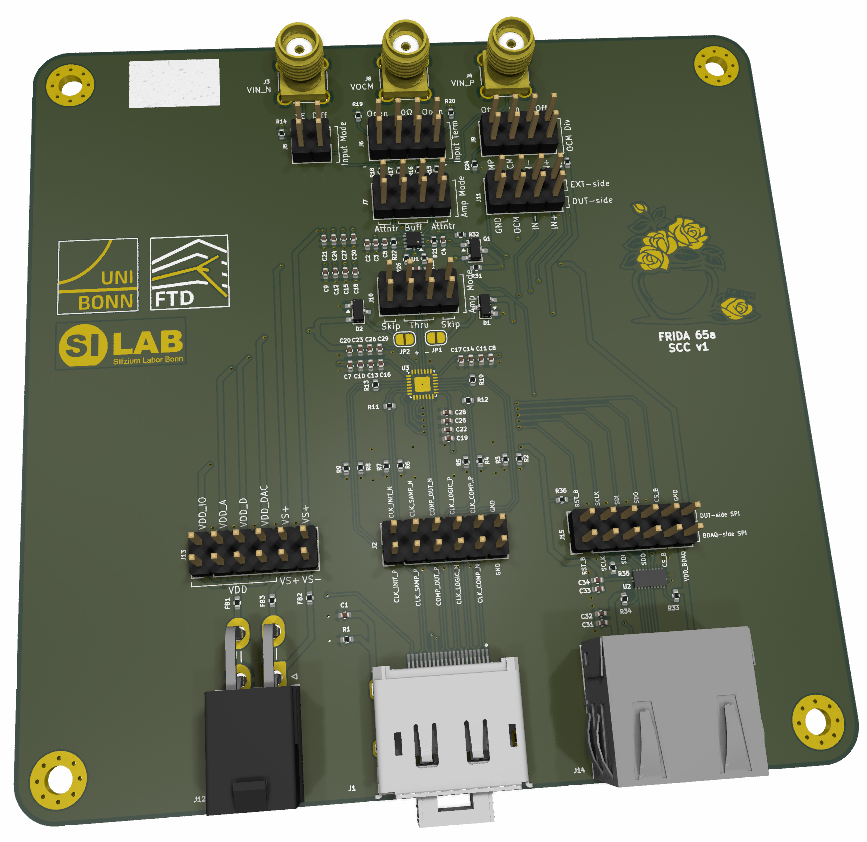
\includegraphics[width=0.96\linewidth,height=0.82\textheight,keepaspectratio]{images/pcb_cropped.png}
\end{frame}

% ============================================================
\begin{frame}
  \frametitle{ADC Channel Variants Across the Array}
  \centering
  \begin{tikzpicture}
    \node[anchor=south west,inner sep=0] (layout) at (0,0)
      {\maybeimage[height=0.82\textheight,keepaspectratio]{images/frida_core.png}};
    % Approximate normalized overlay over the 4x4 ADC array region.
    \begin{scope}[x=0.78\textheight,y=0.82\textheight]
      \foreach \x/\col/\label in {
        0.175/NordBlue/{1L R17},
        0.345/NordGreen/{1L R20},
        0.515/NordOrange/{2L R17},
        0.685/NordPurple/{2L R20}}
      {
        \draw[\col,line width=1.2pt,rounded corners=2pt] (\x,0.26) rectangle +(0.13,0.68);
        \node[\col,fill=white,fill opacity=0.82,text opacity=1,font=\scriptsize\bfseries]
          at (\x+0.065,0.98) {\label};
      }
      \foreach \row/\y in {0/0.86,1/0.70,2/0.54,3/0.38}{
        \foreach \col/\x/\n in {0/0.240/0,1/0.410/1,2/0.580/2,3/0.750/3}{
          \pgfmathtruncatemacro{\adc}{4*\row+\n}
          \node[font=\tiny\bfseries,fill=white,fill opacity=0.80,text opacity=1,inner sep=1.2pt]
            at (\x,\y) {ADC\ifnum\adc<10 0\fi\adc};
        }
      }
    \end{scope}
  \end{tikzpicture}
\end{frame}

% ============================================================
\begin{frame}
  \frametitle{Digital Control and Readout Path}
  \centering
  \maybeimage[width=0.96\linewidth,height=0.46\textheight,keepaspectratio]{images/adc_full.pdf}\\[2pt]
  \maybeimage[width=0.96\linewidth,height=0.46\textheight,keepaspectratio]{images/sequencer_timing.pdf}
\end{frame}

% ============================================================
\begin{frame}
  \frametitle{ADC Schematic and Single-Conversion Simulation}
  \centering
  \maybeimage[width=0.96\linewidth,height=0.46\textheight,keepaspectratio]{images/adc_full.pdf}\\[2pt]
  \maybeimage[width=0.96\linewidth,height=0.46\textheight,keepaspectratio]{images/single_conversion_tspice.png}
\end{frame}

% ============================================================
\begin{frame}
  \frametitle{Transfer Scan: ADC 00, $D_{init}=0101010101010101$}
  \centering
  \maybeimage[width=0.96\linewidth,height=0.82\textheight,keepaspectratio]{../build/basic_scan/adc00_dinit0101010101010101_transfer.png}
\end{frame}

% ============================================================
\begin{frame}
  \frametitle{Code Density: $D_{init}=0101010101010101$}
  \centering
  \maybeimage[width=0.96\linewidth,height=0.82\textheight,keepaspectratio]{../build/basic_scan/adc00_dinit0101010101010101_density.png}
\end{frame}

% ============================================================
\begin{frame}
  \frametitle{DNL/INL: $D_{init}=0101010101010101$}
  \centering
  \maybeimage[width=0.96\linewidth,height=0.82\textheight,keepaspectratio]{../build/basic_scan/adc00_dinit0101010101010101_nonlin.png}
\end{frame}

% ============================================================
\begin{frame}
  \frametitle{Fixed-Input Noise Histogram}
  \centering
  \maybeimage[width=0.88\linewidth,height=0.82\textheight,keepaspectratio]{../build/basic_scan/adc_00_histogram_vinp_1000mV.png}
\end{frame}

% ============================================================
\begin{frame}
  \frametitle{Next Measurement Tasks}
  \begin{itemize}
    \item Check other channels
    \item Better test input-referred noise; currently $>30$ LSB
    \item Vary control-signal phase alignment to check for noise and linearity improvements
    \item Sampling-rate increase; currently $1.25\,\mathrm{MS/s}$
    \item Supply-voltage sweep
    \item ADC calibration: try 2x foreground and 1x background method
  \end{itemize}
\end{frame}

\end{document}
